\documentclass{article}
\usepackage{hyperref}
\usepackage{float}

\begin{document}

\title{Business Ethics of Autonomous Cars}
\author{Kevin Schoonover}

\maketitle

\begin{abstract}
Americans spend on average 308 hours driving~\cite{aaa} and cause on average
35,000 fatalities~\cite{nhtsa_fatalities} every year. The advent of autonomous
cars promises to allow drivers to reclaim these 308 hours while saving over
35,000 lives if implemented perfectly. However, theoretical possibility proved
to be far from reality when autonomous vehicles had a series of fatal crashes
from Uber~\cite{uber} and Tesla~\cite{tesla}. These crashes beg the questions:
`How good must an autonomous car be before an company should release it?' and
`Who is at fault -- the company, the driver, or the other person?'
\end{abstract}

\section{Project}
The project will explore potential answers to the questions by building a web
application that will guide subjects through a series of scenarios and store
their response. The details of the web application will be addressed in the next
section. Then, all results will be condensed and examined in a 1-2 page final
report, not including the data tables.

\subsection{Scenarios}
The \textbf{first scenario} will test the subject on three different stories about
autonomous vehicle crashes. The subject will read a story, select who they think
is at fault (the company, the driver, or the other person), and move onto the
next story. They must choose only one they believe is most at fault.
The stories will be as follows:
\begin{enumerate}
  \item Present the story of the Uber crash presented in~\cite{uber}, but
    anonymize the names and locations to prevent the subject from easily
    recognizing the story.
  \item Present the story of the Tesla crash presented in~\cite{tesla} following
    the same anonymization strategy.
  \item Present a story created by the researcher. This story will contain
    dialog that puts all three potential options into question. An example
    abstract for a story: The company developed a perfect autonomous car;
    however, when it is snowy outside a design flaw makes the car unable to
    detect distant items. The driver fell asleep while traveling to see their
    parents on Christmas (and it was snowing) and signed a licenses agreement
    that the car may not work perfectly in all circumstances. A pedestrian, who
    also cannot see because of the snow, crosses the street and is killed.
\end{enumerate}

The subject will be asked after each question to explain their reasoning of why
they believe each particular person/company is at fault. When the final story is
complete, the user will move on to scenario two.

The \textbf{second scenario} will determine how well an autonomous vehicle needs
to operate before the user will buy it. A series of 5 statements will be
presented that the user will rate from 1 (Highly disagree) to 5 (Strongly
Agree). The statements are as follows:
\begin{itemize}
  \item Autonomous mode must be able to operate in vision impairing rain and/or
    snow.
  \item Autonomous mode must be able to operate during non vision impairing rain
    or snow.
  \item Autonomous mode must be able to operate on a sunny day.
  \item Autonomous mode must be able to operate during the night.
  \item Autonomous mode must work while I am asleep or performing another action.
\end{itemize}

These questions will be asked twice prefaced with the two different modes of
autonomous driving (Fully autonomous and conditional autonomous)\footnote{See
\url{https://cyberlaw.stanford.edu/blog/2013/12/sae-levels-driving-automation}
for more information}. Each definition will be explained before the questions to
give the subject some background. Immediately followed by the subject being
asked to answer from a range of 0-100,000 how many deaths per year is reasonable
for each type of autonomous cars.

\subsection{Web Application}
The web application will have two screens for the different scenarios:
\begin{figure}[H]
\centering
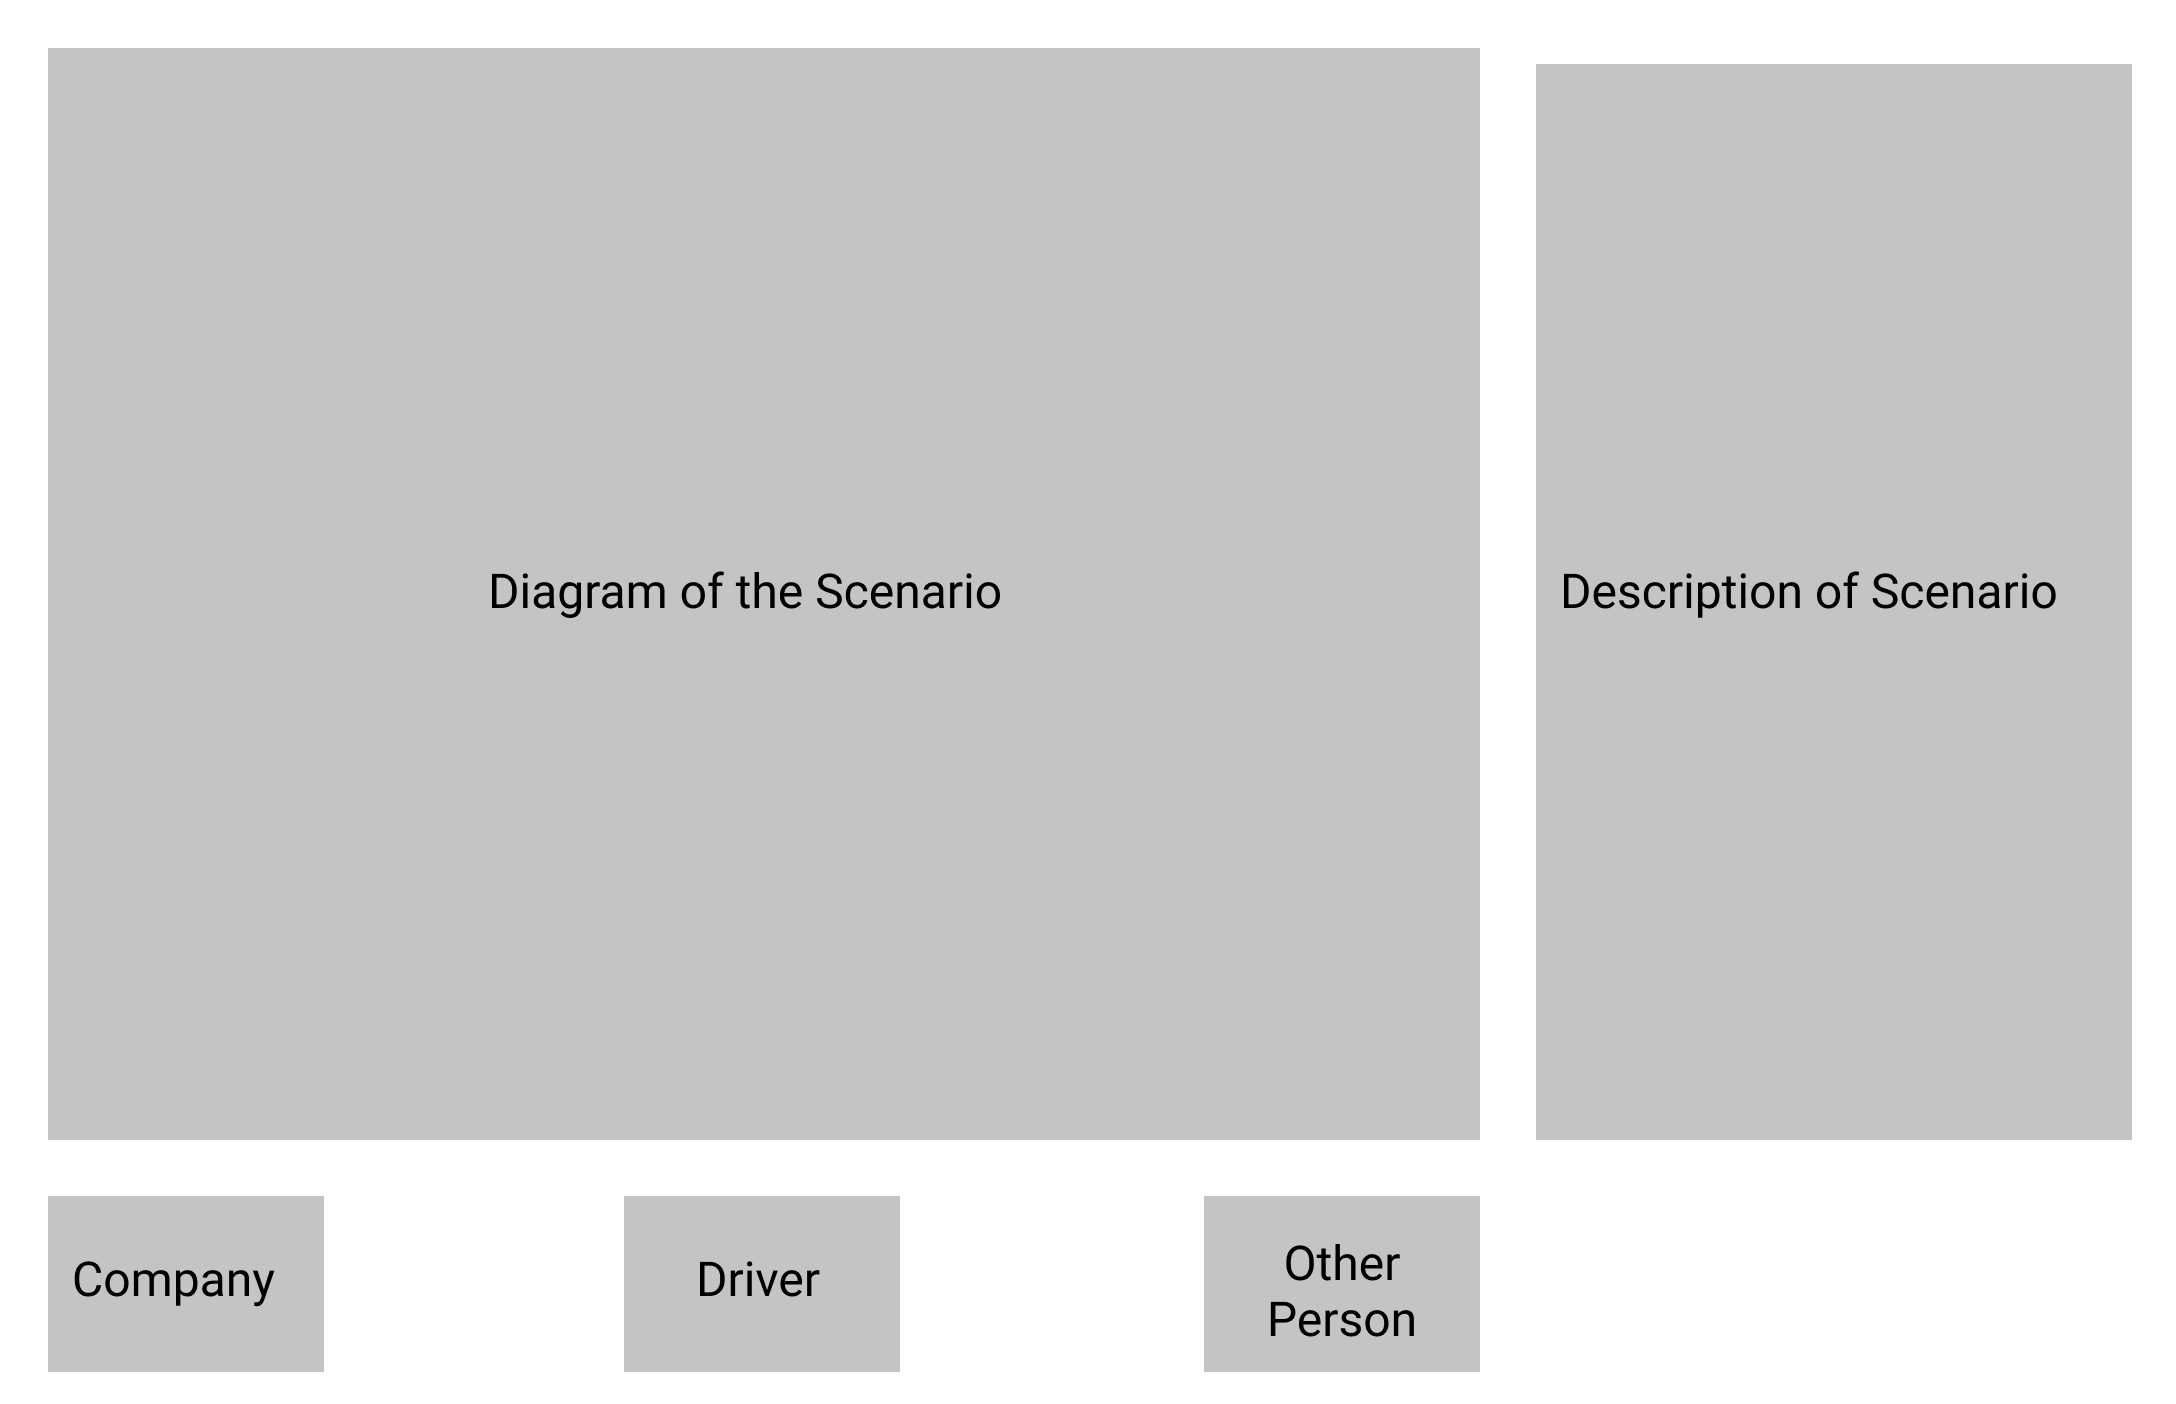
\includegraphics[height=2.5in]{imgs/scenario_1.png}
\caption{Scenario 1 Mock up}
\label{fig:ceads-architecture}
\end{figure}


\subsection{Final Report}

\bibliographystyle{plain}
\bibliography{bib/references}

\end{document}
